\documentclass[12pt,a4paper]{article}
%\usepackage{ctex}
\PassOptionsToPackage{unicode}{hyperref}
\PassOptionsToPackage{hyphens}{url}
\usepackage{amsmath,amscd,amsbsy,amssymb,latexsym,url,bm,amsthm}
\usepackage{epsfig,graphicx,subfigure}
\usepackage{enumitem,balance}
\usepackage{wrapfig}
\usepackage{mathrsfs,euscript}
\usepackage[usenames]{xcolor}
\usepackage[colorlinks,linkcolor = blue]{hyperref}
\usepackage[vlined,ruled,commentsnumbered,linesnumbered]{algorithm2e}
\usepackage{listings}
\usepackage[utf8]{inputenc}
\usepackage{algorithmicx}
\usepackage{algpseudocode}
\usepackage{amsmath}

\newtheorem{theorem}{Theorem}
\newtheorem{lemma}[theorem]{Lemma}
\newtheorem{proposition}[theorem]{Proposition}
\newtheorem{corollary}[theorem]{Corollary}
\newtheorem{exercise}{Exercise}
\newtheorem*{solution}{Solution}
\newtheorem{definition}{Definition}
\theoremstyle{definition}


%\numberwithin{equation}{section}
%\numberwithin{figure}{section}

\renewcommand{\thefootnote}{\fnsymbol{footnote}}

\newcommand{\postscript}[2]
 {\setlength{\epsfxsize}{#2\hsize}
  \centerline{\epsfbox{#1}}}

\renewcommand{\baselinestretch}{1.0}

\setlength{\oddsidemargin}{-0.365in}
\setlength{\evensidemargin}{-0.365in}
\setlength{\topmargin}{-0.3in}
\setlength{\headheight}{0in}
\setlength{\headsep}{0in}
\setlength{\textheight}{10.1in}
\setlength{\textwidth}{7in}
\makeatletter \renewenvironment{proof}[1][Proof] {\par\pushQED{\qed}\normalfont\topsep6\p@\@plus6\p@\relax\trivlist\item[\hskip\labelsep\bfseries#1\@addpunct{.}]\ignorespaces}{\popQED\endtrivlist\@endpefalse} \makeatother
\makeatletter
\renewenvironment{solution}[1][Solution] {\par\pushQED{\qed}\normalfont\topsep6\p@\@plus6\p@\relax\trivlist\item[\hskip\labelsep\bfseries#1\@addpunct{.}]\ignorespaces}{\popQED\endtrivlist\@endpefalse} \makeatother

\SetKwInOut{Input}{Input}
\SetKwInOut{Output}{Output}
\SetKwProg{Fn}{Function}{\string:}{end}

\usepackage{color}
\definecolor{codegreen}{rgb}{0,0.6,0}
\definecolor{codegray}{rgb}{0.5,0.5,0.5}
\definecolor{codepurple}{rgb}{0.58,0,0.82}
\definecolor{backcolour}{rgb}{0.95,0.95,0.92}
 
\lstdefinestyle{mystyle}{  
    commentstyle=\color{codegreen},
    keywordstyle=\color{blue},
    numberstyle=\tiny\color{codegray},
    stringstyle=\color{codepurple},
    basicstyle=\footnotesize,
    breakatwhitespace=false,         
    breaklines=true,                 
    captionpos=b,                    
    keepspaces=true,                 
    numbers=left,                    
    numbersep=5pt,                  
    showspaces=false,                
    showstringspaces=false,
    showtabs=false,                  
    tabsize=2,
    frame=shadowbox
}
\lstset{style=mystyle}

\title{VE477 HW 3}
\author{Wu Jiayao 517370910257}

\begin{document}
\maketitle

\section{}
\subsection{}
    Not done
\subsection{}
    Not done
\subsection{}
\begin{algorithm}[H]
    \BlankLine
    \SetKwFunction{myfunction}{topSorting}	
    \caption{Hamiltonian path problem}
    \Input{A graph $G(V,E)$}
    \Output{Whether there is a Hamiltonian path}
    \Fn{\myfunction{$V$,$E$}}{
        $visitNum$ $\gets$ $0$ \\
        $H$ $\gets$ $\{\}$ \\
        \While{$E$ $\neq$ $\emptyset$}{
            $v$ $\gets$ a vertex in V that no edge points to it \\
            $visitNum++$ \\
            $H[visitNum]$ $\gets$ $v$ \\
            $V$ $\gets$ $V  \backslash v$ \\
            \For {vertex $u$ in $V$}{
                \If{edge $<v,u>$ exists}{
                    $E$ $\gets$ $E \backslash <v,u>$
                }
            }
        }
        \Return $H$ 
    }
    $H$ $\gets$ \myfunction{$V$,$E$} \\
    \For{$i$ in $range(0,len(H))$}{
        \If {$edge<H[i],H[i+1]>$ is not in $E$}{
            \Return false
        }
    }
    \Return true
\end{algorithm}
\subsection{}
    Topological sorting traverses all vertices in $G$. Overall, all edges are traversed for once, since one edge will be removed from $E$ if traversed. Therefore, the complexity is
    $$
        T(n) = \mathcal{O}(V + E)
    $$
\subsection{}
    It is $\mathcal{N} \mathcal{P} \text { -complete }$, as this problem is included in Karp's 21 $\mathcal{NP}$-complete problems.

\section{}
\subsection{}
    It is not bounded by a polynomial.
\subsection{}
Yes.
$$
\log ^{*} n:=\left\{\begin{array}{ll}{0} & {\text { if } n \leq 1} \\ {1+\log ^{*}(\log n)} & {\text { if } n>1}\end{array}\right.
$$
$$
\lim _{n \rightarrow \infty} \frac{\log ^{*} \log n}{\log \log ^{*} n} = \lim _{n \rightarrow \infty} \frac{\log ^{*} n-1}{\log \log ^{*} n} =\lim _{x \rightarrow \infty}\frac{x-1}{\log x} = \infty
$$
\subsection{}
\begin{algorithm}[H]
    \Input{Eight balls with one lighter in weight than each other}
    \Output{The lighter ball}
    Divide into 2 groups of 4 balls. Weight two groups on the balance. Pick out the lighter group of 4 balls. \\
    Divide the lighter group into 2 groups of 2 balls. Weight two groups on the balance. Pick out the lighter group of 2 balls. \\
    Weight the two on the balance. \\
    \Return the lighter ball
\end{algorithm}
\section{}
\par Rubik's Cube is a 3D combination puzzle. On a Rubik's Cube, each of the six faces was covered by nine stickers, with six solid colors. An internal pivot mechanism enables each face to turn independently, thus mixing up the colours. For the puzzle to be solved, each face must be returned to have only one colour for its nine stickers.
\par Two algorithms of solving Rubik's cube are listed as followed.
\newpage
\subsection{}
\begin{enumerate}
    \item Get a white(other color is OK) plus(or cross namely) on the top face. Get the white corner back to the right place to make a whole white face. [Figure~\ref{fig1}]  
        \begin{figure}[h]
            \centering
            \subfigure[White Cross]{
                \begin{minipage}[t]{0.2\linewidth}
                \centering
                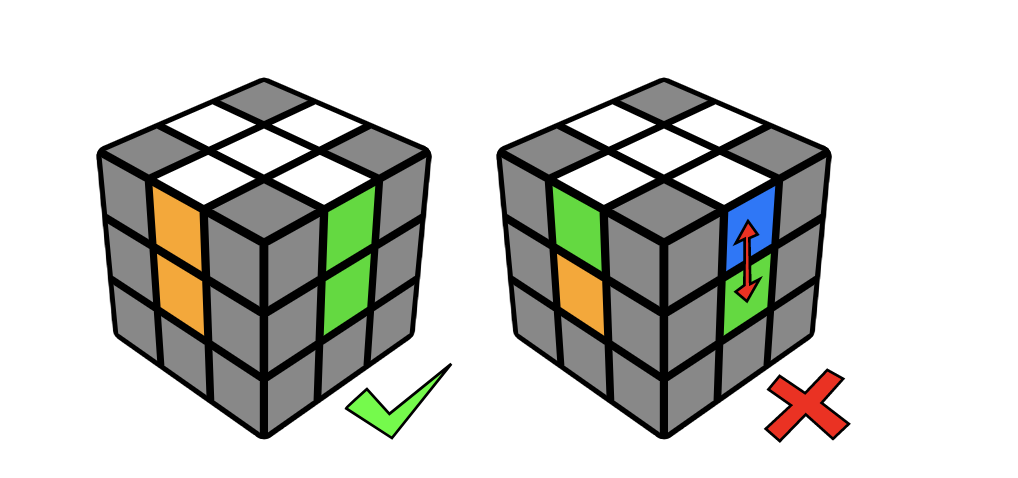
\includegraphics[width=1in]{QQ20191016-095440@2x.png}
                \label{fig1}
                \end{minipage}%
            }%
            \subfigure[Middle Layer's goal]{
                \begin{minipage}[t]{0.2\linewidth}
                \centering
                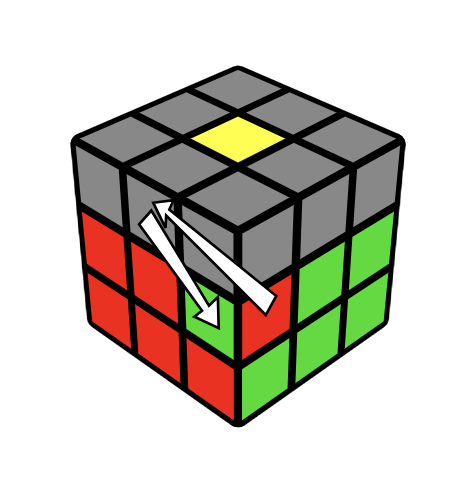
\includegraphics[width=0.7in]{midlayer.png}
                \label{fig2}
                \end{minipage}%
            }%
            \subfigure[Top cross]{
                \begin{minipage}[t]{0.4\linewidth}
                \centering
                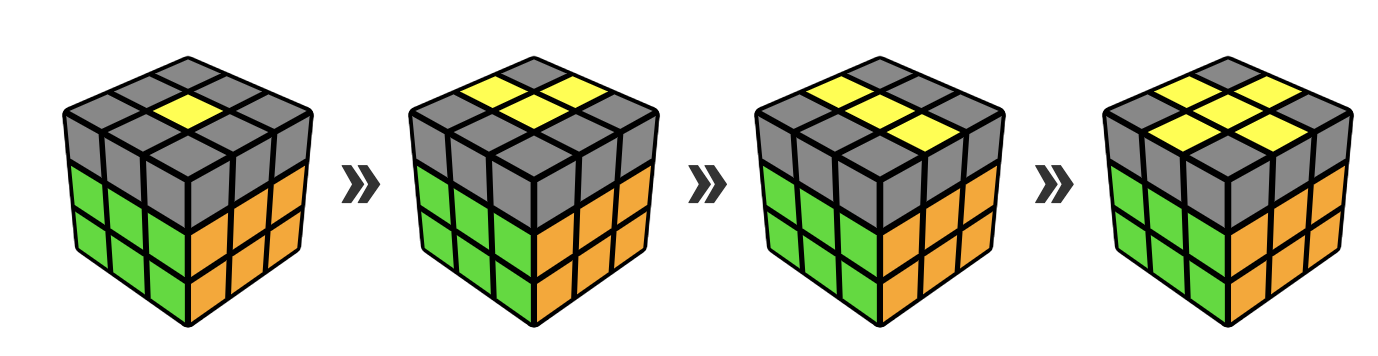
\includegraphics[width=2.6in]{topCross.png}
                \label{fig3}
                \end{minipage}%
            }%
            \subfigure[The goal of Step 4]{
                \begin{minipage}[t]{0.2\linewidth}
                \centering
                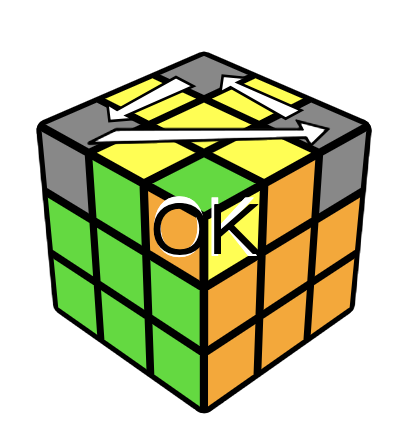
\includegraphics[width=0.7in]{sune.png}
                \label{fig4}
                \end{minipage}%
            }%
        \end{figure}
    \item Flip the cube to make white on the bottom. Get all the pieces in the middle layer to its right place. [Figure~\ref{fig2}] Make the cross on the top face. [Figure~\ref{fig3}] 
    \item By sune and antisune, move four of the yellow cross blocks to its right place that the color of another face of the block matches the color of the cubic's face this face belongs to. [Figure~\ref{fig4}] 
    \item Last, get all the corners of yellow to its right place and right direction.
\end{enumerate}
\subsection{ZZ method}
\begin{enumerate}
    \item This stage orients all edges on the cube (EO) while simultaneously placing the down-front and down-back edges (Line).
    \item It completes the first two layers by building two 1x2x3 blocks on either side of the Line made in the previous step.
    \item Solve the last layer.
\end{enumerate}
{\noindent \bf References}

{\noindent [1] \url{cube3x3.com/%E5%A6%82%E4%BD%95%E8%A7%A3%E5%86%B3%E9%AD%94%E6%96%B9/}}


{\noindent [2] \url{en.wikipedia.org/wiki/Rubik%27s_Cube}}

{\noindent [3] \url{cube.crider.co.uk/zz.php?v=beginner}}

\hrule 
\vskip 2em

\section{}
\subsection{}
    It is $\mathcal{NP}$. Let $y$ be a path in the graph. $\mathcal{O}(\left| V \right| )$ is needed for traverse to verify whether $y$ is a simple path is $True$ 
\subsection{}
    Not done
\subsection{}
    Let $y$ be $k$ vertices in the graph. Then all edges are traversed to test whether each edge contains a vertex cover of size k. The time complexity is $\mathcal{O}(\left| E \right|k)$. Hence, it is $\mathcal{NP}$.
\section{}
It is not sufficient.
Because for an integer $n$, when $n$ becomes bigger, the complexity of division for $n$ is $\log_2n$.
\begin{lstlisting}
int Pos_Div(int x,int y)
{
	int ans=0;
	for(int i=log(n)/log(2);i>=0;i--)
	{
		if((x>>i)>=y)
		{
			ans+=(1<<i);
			x-=(y<<i);
		}
	}
	return ans;
}
\end{lstlisting}
Trial division can be solved in $\mathcal{O}(n)$ if and only if division of n is $\mathcal{O}(1)$, hence trial division is not $\mathcal{O}(n)$. Hence, it is not sufficient to conclude that $PRIME$ is $\mathcal{P}$. \\
By prime number theorem, for a binary base $n$ digits number, the algorithm requires
$$
\pi\left(2^{n / 2}\right) \approx \frac{2^{n / 2}}{\left(\frac{n}{2}\right) \ln 2}
$$
times of division. The time complexity of division is $\mathcal{O}(\log_2(2^n))=\mathcal{O}(n)$. The overall time complexity can be expressed as
$$
    T(n) = \pi\left(2^{n / 2}\right) \times  \mathcal{O}(n) = \mathcal{O}(2^{n / 2})
$$
It is not $\mathcal{P}$.
\end{document}